\section{What a failed run looks like}
\label{sec:phenomenon}

\subsection{Task, data, and model}
\label{sec:phenomenon_arch}

Given the last $w$ observations $X=(x_{t-w+1},\dots,x_t)$ of an engine's
sensor vector $x_t\in\mathbb{R}^{C}$, the RUL task estimates the cycles
remaining before end-of-life. Training labels are counted backwards from the
known failure cycle and clipped at $\bar r=125$, which models the plateau of
incipient degradation. We use the four C-MAPSS subsets
(Table~\ref{tab:datasets}): FD001/FD003 run under one operating condition,
FD002/FD004 under six, and FD003/FD004 add a second fault mode. Because
condition count and fault modes are crossed, an effect seen only on
FD002/FD004 is a multi-condition effect. Constant-variance channels are
dropped, the rest are min--max normalised by training statistics, windows are
split 85/15 into train/validation, and the last window of each test engine is
used for testing.

\begin{table}[t]
\centering\footnotesize
\caption{C-MAPSS subsets and pre-processed sample counts.}
\label{tab:datasets}
\begin{tabularx}{\linewidth}{Xcccccc}
\toprule
Subset & Cond. & Faults & Train eng. & $C$ & Train win. & Test eng. \\
\midrule
FD001 & 1 & 1 & 100 & 17 & 14\,221 & 96 \\
FD002 & 6 & 1 & 260 & 24 & 41\,496 & 259 \\
FD003 & 1 & 2 & 100 & 18 & 18\,547 & 100 \\
FD004 & 6 & 2 & 249 & 24 & 39\,574 & 222 \\
\bottomrule
\end{tabularx}
\end{table}

The hybrid model in Fig.~\ref{fig:arch} is what we study. First-order
differences are concatenated to the raw channels, a $1{\times}1$ convolution
projects to $d=128$, sinusoidal position embeddings and sensor dropout
($0.1$) are applied, five causal dilated TCN blocks (dilations 1--16)
extract local trends, a two-layer BiGRU is added residually, $L$ pre-norm
Transformer layers with 4-head causal attention follow, and an
average/max-pooled MLP head returns a scalar. Window length $w$ and encoder
depth $L$ are the two settings varied below; the full layer specification,
hyperparameters and metric definitions are in Supplementary Section~S1. All
runs use MSE, AdamW ($10^{-4}$), batch 32, cosine annealing over at most 150
epochs and early stopping (patience 20) on validation RMSE, giving
1.08--1.47\,M parameters. A seed controls initialisation and data order; the
validation split is held fixed unless stated otherwise.

\begin{figure*}[t]
\centering
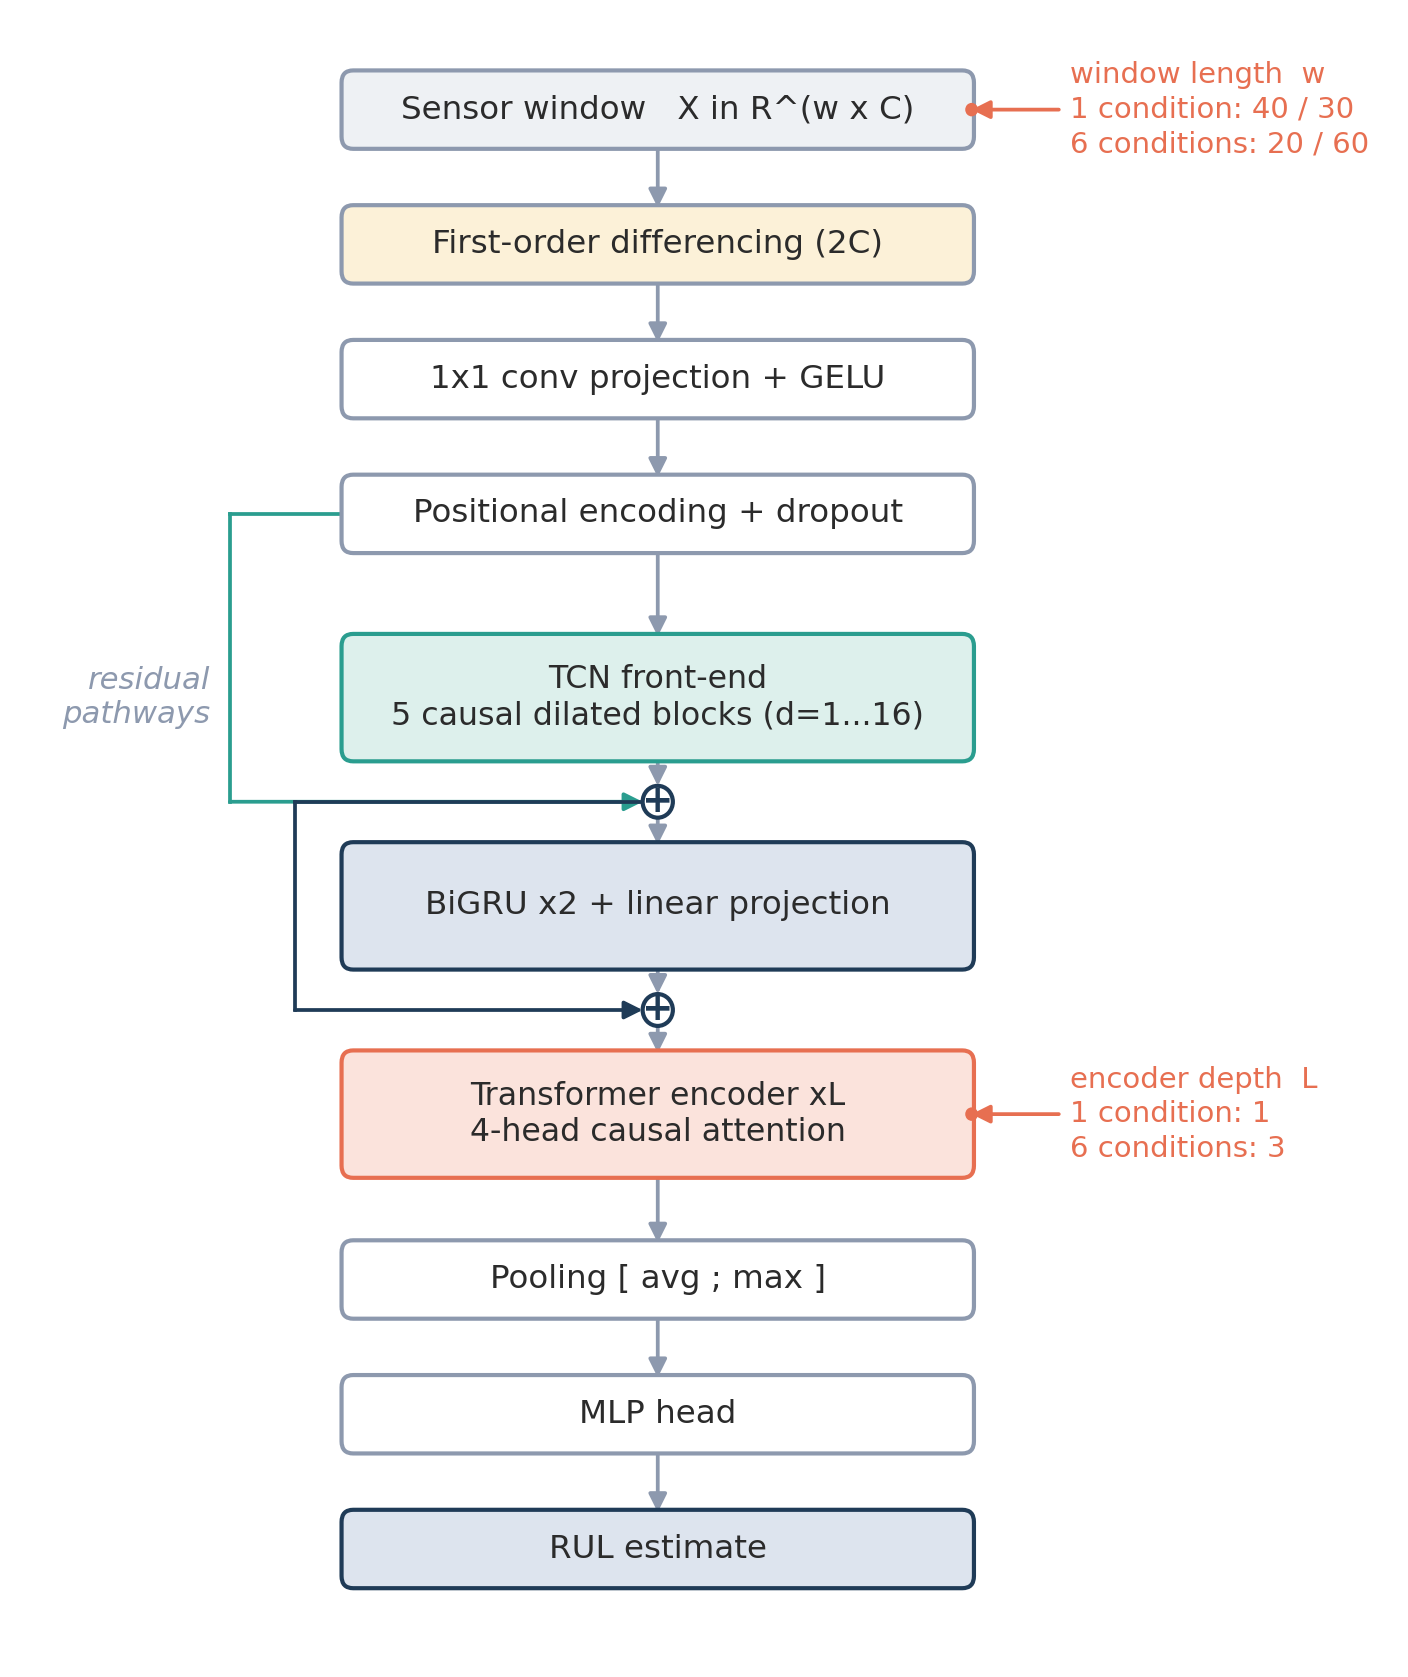
\includegraphics[width=\figarch]{../figures/raster_png_300dpi/fig1_architecture.png}
\caption{The hybrid model studied here. The two red notes give the window
length $w$ and encoder depth $L$ used for one and for six operating
conditions; the small circles mark where a residual branch rejoins the main
path. Section~\ref{sec:mechanism} asks why keeping these branches matters.}
\label{fig:arch}
\end{figure*}

\subsection{Five signs of a failed run}
\label{sec:collapse_def}

Call a run failed when its trained model predicts almost the same number for
every input. Five properties, each checkable from a run log or checkpoint,
identify it: (i) test prediction std $\sigma_{\hat y}<10^{-3}$ cycles, the
constant being 82.57 (FD002) and 82.97--83.00 (FD004); (ii) that constant
equals the training label mean $\bar y_{\mathrm{val}}$ to two decimals
(82.58 / 83.24); (iii) best validation RMSE is reached within 10--15 epochs,
never improves, and equals $\operatorname{std}(y_{\mathrm{val}})$ exactly
(41.97 / 42.24); (iv) because test engines are more degraded than validation
engines ($\bar y_{\mathrm{test}}=73.7$ versus 82.6 on FD002), test RMSE
follows from the label statistics as
\begin{equation}
\mathrm{RMSE}_{\mathrm{failed}}
= \sqrt{\operatorname{Var}(y_{\mathrm{test}})
        + \left(\bar{y}_{\mathrm{val}} - \bar{y}_{\mathrm{test}}\right)^{2}},
\label{eq:fingerprint}
\end{equation}
derived in Supplementary Section~S8; and (v) per-RUL-bucket errors follow the
constant prediction (69.9 / 38.5 / 10.7 / 38.2 on FD002).
Table~\ref{tab:fingerprint} checks (iv) against every failed run in the
archive: the prediction is accurate to 0.01 cycles on both subsets, so these
runs all end up at the same output rather than at a range of bad solutions.
Failed runs also give nearly identical RMSE across unrelated configurations
(43.848, 43.847, 43.846 for three depths and two GRL variants on FD002).
Losses fall smoothly, gradients behave and early stopping triggers normally,
so a reported ``RMSE = 43.85'' reads as poor tuning rather than as a distinct
failure. With one seed, a configuration that often fails cannot be told apart
from one that is simply mediocre.

\begin{table}[t]
\centering\footnotesize
\caption{A formula for the error of a failed run: observed versus predicted
RMSE (Eq.~(\ref{eq:fingerprint})).}
\label{tab:fingerprint}
\begin{tabularx}{\linewidth}{XCCCC}
\toprule
Subset & Std.\ $y_{\mathrm{val}}$ & Best-val & Constant pred./obs. &
Eq.~(\ref{eq:fingerprint}) / obs. \\
\midrule
FD002 & 41.97 & 41.97 & 82.58 / 82.57 & 43.85 / 43.85 \\
FD004 & 42.24 & 42.24 & 83.24 / 82.97--83.00 & 43.71 / 43.67--43.71 \\
\bottomrule
\end{tabularx}
\end{table}

\begin{figure}[t]
\centering
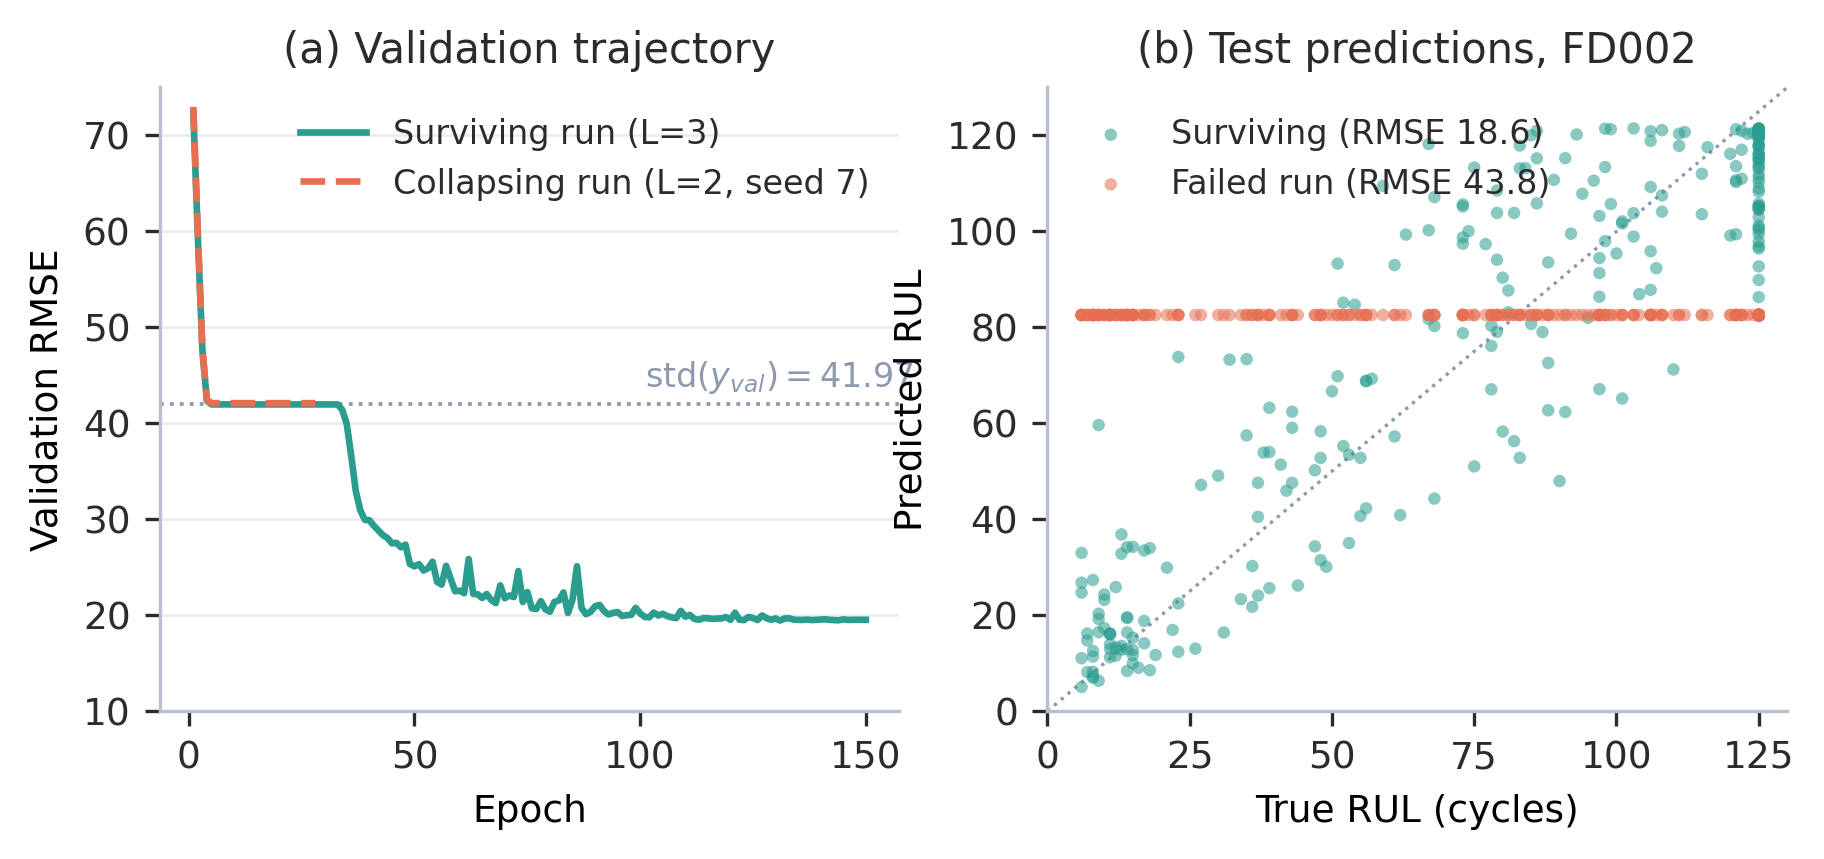
\includegraphics[width=0.68\linewidth]{../figures/raster_png_300dpi/fig2_fingerprint.png}
\caption{What a failed run looks like. (a) Validation RMSE of a working and
a failing FD002 run ($L{=}2$, seed 7): both sit at
$\operatorname{std}(y_{\mathrm{val}})$ for many epochs, and only the former
starts improving again near epoch 34. (b) Test predictions versus true RUL:
the failed model emits 82.6 for every engine.}
\label{fig:fingerprint_scatter}
\end{figure}

\subsection{How often it happens}
\label{sec:prevalence}

We audited all 161 archived runs, spanning $w\in\{20,30,40,60\}$,
$L\in\{1,\dots,4\}$, heads $h\in\{2,4,8\}$, three placements of adversarial
(GRL) regularisation and their controls; a run counts as failed iff test
RMSE $>40$, which Section~\ref{sec:collapse_def} shows to be conservative.
None of the 81 single-condition runs failed, including deliberately
pathological configurations (Table~\ref{tab:prevalence}). On multi-condition
data, failures gather in a few settings: in the controlled depth search
FD002 $L\in\{2,4\}$ failed while $L\in\{1,3\}$ trained normally, and the
order reversed on FD004 ($L{=}1$ failed, $L\geq2$ worked); window size and
head count behave similarly (FD002 with the adversarial backbone:
$w\in\{30,60\}$ failed, $w\in\{20,40\}$ did not; $h{=}2$ failed where
$h{=}4,8$ did not). Whether training works is a property of the dataset and
the architecture together, not of depth or window size alone. The complete
grids are in Supplementary Table~S2 and Fig.~S1.

\begin{table}[t]
\centering\footnotesize
\caption{How often runs failed on each subset (161 archived runs; four runs
with no recorded subset label are omitted from the breakdown).}
\label{tab:prevalence}
\begin{tabularx}{\linewidth}{Xccc}
\toprule
Subset & Runs & Failed & Rate \\
\midrule
FD001 (1 condition) & 45 & 0 & 0\% \\
FD003 (1 condition) & 36 & 0 & 0\% \\
FD002 (6 conditions) & 43 & 16 & 37.2\% \\
FD004 (6 conditions) & 33 & 8 & 24.2\% \\
\bottomrule
\end{tabularx}
\end{table}

The FD004 $w{=}60$, $L{=}3$ configuration has been trained under eight seeds:
six failed (43.67--43.72, each matching Eq.~(\ref{eq:fingerprint}) to two
decimals) and two worked (19.46, 19.60), with no intermediate outcome. The
two working runs form the tightest accuracy cluster in the archive (std
0.07), so one configuration can give first-quartile accuracy and still fail
on three retrains out of four. GRL variants shift which settings fail
without removing the problem, and seeded re-runs of archived failure cells
show that the seed, not the configuration alone, often decides the outcome
(Section~\ref{sec:dynamics}). How often a configuration fails therefore has
to be measured over seeds, as the audit of Section~\ref{sec:method_audit}
does. Published C-MAPSS results report one run per configuration;
best-of-$k$ tuning or reporting only the run that worked hides this.
